\documentclass[a4paper,9pt]{extarticle}
\usepackage[dutch]{babel}
% Package to make citations superscrit with brackets
\usepackage[super,square]{natbib}
\RequirePackage{times}
\usepackage[scaled]{inconsolata}
\usepackage{graphicx} 
\usepackage{titlesec}
\usepackage{amsmath}
\usepackage[hypcap=true]{caption}  % of report, book, etc.
\titleformat{\section}
  {\normalfont\LARGE\bfseries}
  {\thesection}{1em}{}  



% Package to change margin size
\usepackage{anysize}
\marginsize{1.5cm}{1.5cm}{1cm}{1cm}

\usepackage{lastpage}

\usepackage{listings}
% Package to make headers


\usepackage{xcolor}
% Kleuren gebaseerd op je screenshot
\definecolor{codepurple}{RGB}{153, 0, 102}     
\definecolor{codeorange}{RGB}{0, 0, 0}         
\definecolor{codeblue}{RGB}{0, 0, 0}           
\definecolor{codegreen}{RGB}{0, 128, 0}        
\definecolor{codegray}{RGB}{0, 0, 0}  
\definecolor{codedarkblue}{RGB}{0, 0, 139}        % 

 % iets grijzer achtergrond
\definecolor{background}{RGB}{255, 255, 255}  
% donkergrijze tekst
\lstset{
  language=Python,
  backgroundcolor=\color{background},
  basicstyle=\ttfamily\small\color{codegray},
  numbers=left,
  numberstyle=\tiny\color{gray},
  numbersep=7pt,
  frame=single,
  framesep=2pt,
  rulecolor=\color{codegray},
  keywordstyle=\color{codepurple},
  stringstyle=\color{codeorange},
  identifierstyle=\color{codeblue},
  commentstyle=\color{codegreen},
  moredelim=[s][\color{codegreen}]{"""}{"""},
  showstringspaces=false,
  aboveskip=1em,
  belowskip=1em,
  breaklines=true,
  breakatwhitespace=true,
  emph={build_feedforward_model},
  emphstyle=\color{codedarkblue},
}
\usepackage{fancyhdr}
\renewcommand{\headrulewidth}{0pt}
\cfoot{}
% Package for highligths
\usepackage{soul}
% Colors for the references links
\usepackage[dvipsnames]{xcolor}
% Package to link references
\usepackage{hyperref}
\hypersetup{
    colorlinks=true,
    linkcolor=black,
    citecolor=CadetBlue,
    filecolor=CadetBlue,      
    urlcolor=CadetBlue,
}
% Package for lorem ipsum
\usepackage{lipsum}
% Package for multicolumn
\usepackage{multicol}
% Package for removing paragraph identations
\usepackage{parskip}
\setlength\columnsep{18pt}
% Sets bastract
\renewenvironment{abstract}
 {\par\noindent\textbf{Samenvatting}\ \ignorespaces \\}
 {\par\noindent\medskip}

\begin{document}
% Makes header
\pagestyle{fancy}
\fancyhead[R]{\textit{PEE51}}
\fancyhead[C]{\textit{Elektrotechniek}}
\fancyhead[L]{\textit{Hogeschool Rotterdam}}
\fancyfoot[L]{M. Reints}
\fancyfoot[C]{}
\fancyfoot[R]{pagina \thepage\ van \pageref{LastPage}}
% Makes footnotes with an asterisk
\renewcommand*{\thefootnote}{\fnsymbol{footnote}}
\begin{center}
  \huge{\textbf{Stap-voor-stap Handleiding: Neuraal Netwerk in TensorFlow}} \\
  \vspace{0.2cm}
  \large{Uitleg en toelichting op Python-code voor het ontwikkelen van een AI-regelaar ter vervanging van een PID-systeem}
\vspace{0.2cm}
\normalsize
\\ Mitchel Reints - \href{mailto:1040953@hr.nl}{1040953@hr.nl} \\
\vspace{0.1cm}
\textit{Hogeschool Rotterdam - Elektrotechniek - PEE51} 
\vspace{0.1cm} \\
\today
\medskip
\normalsize
\end{center}

{\color{gray}\hrule}
\begin{multicols}{2}
\setlength{\headheight}{14.49998pt}
\titleformat{\section}
  {\normalfont\LARGE\bfseries\centering}
  {\thesection}{1em}{}  
%\tableofcontents

\section{introductie}
In deze handleiding wordt stap voor stap uitgelegd hoe het neuraal netwerk voor PEE51 project is opgesteld. Dit project is een onderdeel van de opleiding Elektrotechniek aan de Hogeschool Rotterdam. Het doel van deze handleiding is om stap voor stap uit te leggen hoe een neuraal netwerk ontwikkeld, getraind en geëvalueerd kan worden in Python met TensorFlow. Dit netwerk is bedoeld om het gedrag van een klassieke PID-regelaar na te bootsen of te verbeteren in een systeem waarbij een pingpongbal op een ingestelde hoogte wordt gehouden door middel van een ventilator. De aanpak richt zich op het bouwen van een werkend AI-model, met als einddoel het inzetten van dit model op een embedded platform. Daarbij ligt de nadruk op nauwkeurige en stabiele hoogtecontrole, net als bij de bestaande PID-regeling.  In deze handleiding wordt uitsluitend ingegaan op de technische implementatie van het neuraal netwerk; aspecten zoals gebruikersinterface, documentatie of demonstratieopstelling blijven buiten beschouwing. Voor meer informatie over het prestatieonderzoek en de vergelijking met de PID-regelaar, zie het bijbehorende onderzoeksrapport: \url{https://example.com/onderzoek-ai-regelaar}.
\setlength{\headheight}{14.49998pt}
\titleformat{\section}
  {\normalfont\LARGE\bfseries\centering}
  {\thesection}{1em}{}  
%\tableofcontents

\section{Benodigheden}
Voor dat we aan de slag kunnen met het neuraal netwerk, zijn er een aantal benodigdheden die we moeten installeren. Voor het installeren van de juiste packages en het opzetten van de omgeving, is het belangrijk om te zorgen dat je de juiste versie van Python en de benodigde bibliotheken hebt. De handleiding gaat ervan uit dat je bekend bent met de basisprincipes van Python en hoe je een Python-omgeving kunt opzetten. Als je nog niet bekend bent met Python, raden we aan om eerst een introductiecursus te volgen of de officiële documentatie te lezen. Deze benodigdheden zijn:

Deze benodigdheden zijn essentieel voor het ontwikkelen, trainen en evalueren van het neuraal netwerk. Hieronder worden deze benodigdheden kort toegelicht:
\begin{itemize}
  \item \textbf{Python 3.10 of hoger:} De programmeertaal waarin het neuraal netwerk wordt ontwikkeld. Zorg ervoor dat je de nieuwste versie van Python hebt geïnstalleerd.
  \item \textbf{TensorFlow 2.11 of hoger:} Een populaire open-source bibliotheek voor machine learning en deep learning, die wordt gebruikt om neurale netwerken te bouwen en te trainen.
  \item \textbf{NumPy:} Een fundamentele bibliotheek voor wetenschappelijk rekenen in Python, die wordt gebruikt voor het werken met arrays en wiskundige functies.
  \item \textbf{Matplotlib:} Een bibliotheek voor het maken van visualisaties in Python, die nuttig is voor het plotten van resultaten en het visualiseren van data.
  \item \textbf{Jupyter Notebook (optioneel):} Een interactieve omgeving voor het schrijven en uitvoeren van Python-code, die handig is voor het ontwikkelen en testen van het neuraal netwerk.
  \item \textbf{Een teksteditor of IDE:} Een omgeving waarin je de Python-code kunt schrijven en uitvoeren. Populaire keuzes zijn Visual Studio Code, PyCharm of Jupyter Notebook.

\end{itemize}

Tijdens het doorlopen van de stappen in deze handleiding worden alle geïmporteerde pakketten en hun toepassing in de code uitvoerig toegelicht, zodat duidelijk wordt waarom elk pakket nodig is.
\subsection*{Versies van gebruikte pakketten}
Voor dit project zijn de volgende pakketversies gebruikt om compatibiliteit en reproduceerbaarheid te waarborgen:
\begin{itemize}
  \item \textbf{Pandas:} 2.2.3
  \item \textbf{NumPy:} 1.26.4
  \item \textbf{Matplotlib:} 3.10.1
  \item \textbf{TensorFlow:} 2.15.0
  \item \textbf{Keras:} 2.15.0
\end{itemize}

De onderstaande pakketten zijn in dit project gebruikt en worden in de code geïmporteerd. Zorg ervoor dat je ze allemaal installeert voordat je aan de slag gaat:
\begin{itemize}
  \item \textbf{pandas, numpy, matplotlib:} voor data-analyse en visualisatie
  \item \textbf{tensorflow, keras:} voor het bouwen, trainen en evalueren van het neuraal netwerk
  \item \textbf{scikit-learn:} voor dataset splitsing en normalisatie
\end{itemize}
Hieronder staat een voorbeeld van de benodigde imports in Python. Deze code moet aan het begin van je Python-script of Jupyter Notebook worden toegevoegd om de benodigde bibliotheken te importeren:
\begin{lstlisting}[language=Python, numbers=left, breaklines=true, basicstyle=\ttfamily\scriptsize]
import pandas as pd
import numpy as np
import matplotlib.pyplot as plt
import tensorflow as tf
from tensorflow import keras
from keras import layers, models, callbacks, preprocessing
from sklearn.model_selection import train_test_split 
from keras.layers import Input, Dense, Conv1D, Flatten
from keras.models import Model, Sequential
from sklearn.preprocessing import MinMaxScaler
import keras
\end{lstlisting}

\setlength{\headheight}{14.49998pt}
\titleformat{\section}
  {\normalfont\LARGE\bfseries\centering}
  {\thesection}{1em}{}  
%\tableofcontents

\section{datavoorbereiden}
In deze sectie wordt stap voor stap uitgelegd hoe de data wordt voorbereid voor het trainen van het neuraal netwerk. De data bestaat uit een CSV-bestand met de volgende kolommen: tijd, hoogte, snelheid, en ventilatorsnelheid. 


\begin{lstlisting}[language=Python, numbers=left, breaklines=true, basicstyle=\ttfamily\scriptsize]
CSV_PATH = '/Users/username/Documents/PEE51/data/data.csv'
CSV_DATA = pd.read_csv(CSV_PATH)
# Toon aantal samples
total_samples = len(CSV_DATA)
\end{lstlisting}

\begin{lstlisting}[language=Python, numbers=left, breaklines=true, basicstyle=\ttfamily\scriptsize]
# Selecteer features en target
features = CSV_DATA[['Setpoint (m)', 'Hoogte (m)', 'Fout', 'Fout_Integratie', 'Fout_Afgeleide']].to_numpy()
target = CSV_DATA['PWM'].to_numpy()
\end{lstlisting}


\begin{lstlisting}[language=Python, numbers=left, breaklines=true, basicstyle=\ttfamily\scriptsize]
n_input = 2  # aantal tijdstappen per voorbeeld

X, y = [], []

for i in range(len(features) - n_input):
    X.append(features[i:i + n_input])
    y.append(target[i + n_input])  # de PWM bij het volgende moment

X = np.array(X)  # shape: (samples, n_input, features)
y = np.array(y)

print("X shape:", X.shape)  # (samples, tijdstappen, features)
print("y shape:", y.shape)  # (samples,)
print("X:", X)  # (samples, tijdstappen, features)
print("y:", y) 
\end{lstlisting}

\end{multicols}
\setlength{\headheight}{14.49998pt}
\titleformat{\section}
  {\normalfont\LARGE\bfseries\centering}
  {\thesection}{1em}{}  
%\tableofcontents

\section{Model bouwen en compileren}




\begin{lstlisting}[language=Python, numbers=left, breaklines=true, basicstyle=\ttfamily\scriptsize]
model = Sequential([
    Conv1D(filters=32, kernel_size=2, activation='relu', input_shape=(n_input, X.shape[2])),
    Flatten(),
    Dense(64, activation='relu'),
    Dense(1)  # Één PWM-waarde voorspellen
])

model.summary()
\end{lstlisting}

\begin{lstlisting}[language=Python, numbers=left, breaklines=true, basicstyle=\ttfamily\scriptsize]
model = Sequential([
    Conv1D(filters=32, kernel_size=2, activation='relu', input_shape=(n_input, X.shape[2])),
    Flatten(),
    Dense(64, activation='relu'),
    Dense(1)  # Één PWM-waarde voorspellen
])

model.summary()
\end{lstlisting}




\setlength{\headheight}{14.49998pt}
\titleformat{\section}
  {\normalfont\LARGE\bfseries\centering}
  {\thesection}{1em}{}  
%\tableofcontents

\section{Model compileren}



\setlength{\headheight}{14.49998pt}
\titleformat{\section}
  {\normalfont\LARGE\bfseries\centering}
  {\thesection}{1em}{}  
%\tableofcontents

\section{Model trainen}



\setlength{\headheight}{14.49998pt}
\titleformat{\section}
  {\normalfont\LARGE\bfseries\centering}
  {\thesection}{1em}{}  
%\tableofcontents

\section{Model evalueren}



\setlength{\headheight}{14.49998pt}
\titleformat{\section}
  {\normalfont\LARGE\bfseries\centering}
  {\thesection}{1em}{}  
%\tableofcontents

\section{model opslaan/exporteren}



\bibliographystyle{plain}
\bibliography{references}
\section*{Begrippenlijst}
\begin{description}
  \item[PID-regelaar] Een regelsysteem dat gebruikmaakt van proportionele, integrale en afgeleide termen.
  \item[Neuraal netwerk] Een algoritme geïnspireerd op het menselijk brein dat patronen leert herkennen.
  \item[Backpropagation] Methode om foutmarges in een neuraal netwerk terug te voeren en gewichten aan te passen.
\end{description}
For more details, refer to \cite{Bowker1985}.
\titleformat{\section}
  {\normalfont\LARGE\bfseries}
  {\thesection}{1em}{} 

\appendix
\section{Meetresultaten}
\label{appendix:meetresultaten}

In deze bijlage worden de meetresultaten weergegeven die zijn verzameld tijdens de experimenten.

\section{Tabel met resultaten}
Hieronder staat een overzichtstabel van de gemeten waarden.

\begin{table}[h!]
\centering
\begin{tabular}{|c|c|c|}
\hline
Tijd (s) & Spanning (V) & Stroom (A) \\
\hline
0.0 & 3.30 & 0.10 \\
1.0 & 3.28 & 0.11 \\
2.0 & 3.27 & 0.12 \\
\hline
\end{tabular}
\caption{Gemeten waarden tijdens test 1}
\end{table}

\section{Grafiek}
Hier zie je een voorbeeld van een grafiek (je moet je eigen figuur invoegen):

\begin{figure}[h!]
\centering
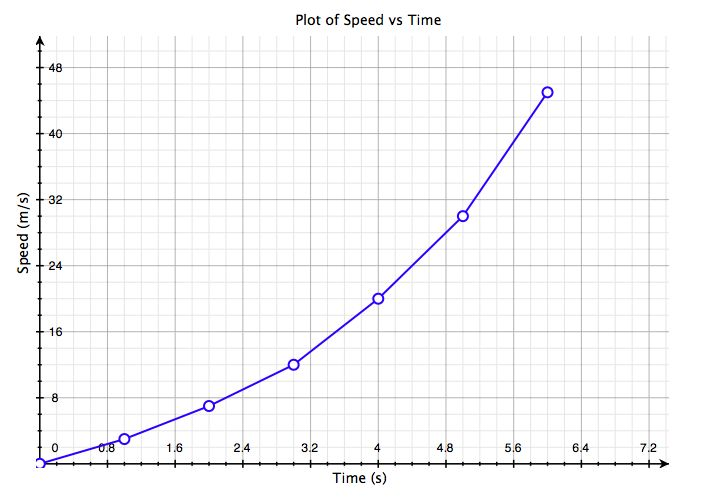
\includegraphics[width=0.7\textwidth]{./afbeeldingen/grafiek.jpeg}
\caption{Spanning over tijd}
\label{fig:spanning_tijd}
\end{figure}

\section{Broncode}
\label{appendix:broncode}

\section{python-script}
\begin{lstlisting}[language=Python, numbers=left, breaklines=true, basicstyle=\ttfamily\scriptsize]
    def build_feedforward_model(input_layer_size, hidden_layer_size, output_layer_size):
        """Bouw een neuraal netwerkmodel volgens TensorFlow-conventies."""
        model = keras.Sequential(name="Feedfoward_Model")
        model.add(layers.Input(shape=(input_layer_size,), name="Input_Layer"))
        model.add(layers.Dense(hidden_layer_size, activation='sigmoid', name="Hidden_Layer"))
        model.add(layers.Dense(hidden_layer_size_2, activation='sigmoid', name="Hidden_Layer_2"))
        model.add(layers.Dense(output_layer_size, activation='softmax', name="Output_Layer"))
        return model 
\end{lstlisting}
 
\end{document}